% Options for packages loaded elsewhere
\PassOptionsToPackage{unicode}{hyperref}
\PassOptionsToPackage{hyphens}{url}
\documentclass[
  ignorenonframetext,
]{beamer}
\newif\ifbibliography
\usepackage{pgfpages}
\setbeamertemplate{caption}[numbered]
\setbeamertemplate{caption label separator}{: }
\setbeamercolor{caption name}{fg=normal text.fg}
\beamertemplatenavigationsymbolsempty
% remove section numbering
\setbeamertemplate{part page}{
  \centering
  \begin{beamercolorbox}[sep=16pt,center]{part title}
    \usebeamerfont{part title}\insertpart\par
  \end{beamercolorbox}
}
\setbeamertemplate{section page}{
  \centering
  \begin{beamercolorbox}[sep=12pt,center]{section title}
    \usebeamerfont{section title}\insertsection\par
  \end{beamercolorbox}
}
\setbeamertemplate{subsection page}{
  \centering
  \begin{beamercolorbox}[sep=8pt,center]{subsection title}
    \usebeamerfont{subsection title}\insertsubsection\par
  \end{beamercolorbox}
}
% Prevent slide breaks in the middle of a paragraph
\widowpenalties 1 10000
\raggedbottom
\AtBeginPart{
  \frame{\partpage}
}
\AtBeginSection{
  \ifbibliography
  \else
    \frame{\sectionpage}
  \fi
}
\AtBeginSubsection{
  \frame{\subsectionpage}
}
\usepackage{iftex}
\ifPDFTeX
  \usepackage[T1]{fontenc}
  \usepackage[utf8]{inputenc}
  \usepackage{textcomp} % provide euro and other symbols
\else % if luatex or xetex
  \usepackage{unicode-math} % this also loads fontspec
  \defaultfontfeatures{Scale=MatchLowercase}
  \defaultfontfeatures[\rmfamily]{Ligatures=TeX,Scale=1}
\fi
\usepackage{lmodern}
\ifPDFTeX\else
  % xetex/luatex font selection
\fi
% Use upquote if available, for straight quotes in verbatim environments
\IfFileExists{upquote.sty}{\usepackage{upquote}}{}
\IfFileExists{microtype.sty}{% use microtype if available
  \usepackage[]{microtype}
  \UseMicrotypeSet[protrusion]{basicmath} % disable protrusion for tt fonts
}{}
\makeatletter
\@ifundefined{KOMAClassName}{% if non-KOMA class
  \IfFileExists{parskip.sty}{%
    \usepackage{parskip}
  }{% else
    \setlength{\parindent}{0pt}
    \setlength{\parskip}{6pt plus 2pt minus 1pt}}
}{% if KOMA class
  \KOMAoptions{parskip=half}}
\makeatother
\usepackage{graphicx}
\makeatletter
\newsavebox\pandoc@box
\newcommand*\pandocbounded[1]{% scales image to fit in text height/width
  \sbox\pandoc@box{#1}%
  \Gscale@div\@tempa{\textheight}{\dimexpr\ht\pandoc@box+\dp\pandoc@box\relax}%
  \Gscale@div\@tempb{\linewidth}{\wd\pandoc@box}%
  \ifdim\@tempb\p@<\@tempa\p@\let\@tempa\@tempb\fi% select the smaller of both
  \ifdim\@tempa\p@<\p@\scalebox{\@tempa}{\usebox\pandoc@box}%
  \else\usebox{\pandoc@box}%
  \fi%
}
% Set default figure placement to htbp
\def\fps@figure{htbp}
\makeatother
\setlength{\emergencystretch}{3em} % prevent overfull lines
\providecommand{\tightlist}{%
  \setlength{\itemsep}{0pt}\setlength{\parskip}{0pt}}
% Slide layout defaults for warning-clean scientific decks.
\usepackage{etoolbox}
\IfFileExists{xurl.sty}{\usepackage{xurl}}{}
\IfFileExists{seqsplit.sty}{\usepackage{seqsplit}}{\newcommand{\seqsplit}[1]{#1}}
\protected\def\breakseq#1{\seqsplit{#1}}
\protected\def\breaktt#1{\begingroup\ttfamily\seqsplit{#1}\endgroup}
\setlength{\emergencystretch}{6em}
\tolerance=5000
\hbadness=10000
\hfuzz=1pt
\setlength{\tabcolsep}{2pt}
\AtBeginEnvironment{longtable}{\tiny\renewcommand{\arraystretch}{0.86}\setlength{\tabcolsep}{1pt}}
\AtBeginEnvironment{tabular}{\tiny\renewcommand{\arraystretch}{0.86}\setlength{\tabcolsep}{1pt}}

% Natbib and cross-reference fallbacks — slides don't load natbib
% or cleveref, but combined-PDF manuscript prose may emit these
% commands. The fallback renders citations as a bracketed key list
% and cross-references as detokenized labels so slides don't fail on
% undefined control sequences or raw underscores. \providecommand is
% a no-op if packages load later.
\providecommand{\citep}[1]{[#1]}
\providecommand{\citet}[1]{#1}
\providecommand{\citealp}[1]{#1}
\providecommand{\citeauthor}[1]{#1}
\providecommand{\citeyear}[1]{#1}
\providecommand{\cref}[1]{\texttt{\detokenize{#1}}}
\providecommand{\Cref}[1]{\texttt{\detokenize{#1}}}

\newtheorem{proposition}{Proposition}
\newtheorem{hypothesis}{Hypothesis}
\usepackage{bookmark}
\IfFileExists{xurl.sty}{\usepackage{xurl}}{} % add URL line breaks if available
\urlstyle{same}
% fallback for those not using the hyperref driver hyperxmp:
\makeatletter
\@ifundefined{xmpquote}{\newcommand{\xmpquote}[1]{#1}}{}
\makeatother
\hypersetup{
  hidelinks,
  pdfcreator={LaTeX via pandoc}}

\author{\texorpdfstring{}{}}
\date{}

\begin{document}

\section{Cyberphysical Substrate: Canvas, Body,
Archive}\label{sec:cyberphysical}

\begin{frame}[fragile,allowframebreaks]{Cyberphysical Substrate: Canvas,
Body, Archive}
Cyberphysical DigiPPPiP treats the ``paper'' in PPPiP as a variable
substrate rather than a fixed object. Pen-and-paper remains the haptic
baseline, but shared tablets, web canvases, augmented reality (AR)
overlays, virtual reality (VR) drawing spaces, smart paper, and
persistent whiteboards all create different couplings among gesture,
mark, archive, and partner response. Cyber-physical-social systems
(CPSS) research is useful because it keeps physical, cyber, and social
layers in one analytic frame rather than reducing the system to a device
or app \breakseq{[@sobb2023cpss]}. Collaborative-work studies add a second
discipline: the drawing surface must preserve the interactional value of
gestures, spatial relations, and work-in-progress marks, not only the
final image \breakseq{[@tang1991collaborativework; @ishii1993clearboard]}.

That design discipline is stronger when the canvas is treated as a
shared-workspace system rather than as a drawing file with two accounts.
Workspace awareness asks what each partner can know about the other's
location, action, intention, and change history in the shared field
\breakseq{[@gutwin2002workspaceawareness]}. Social translucence asks whether
that visibility supports social coordination and accountability without
becoming total visibility \breakseq{[@erickson2000socialtranslucence]}.
Collaborative tabletop research adds a spatial constraint: people create
personal, group, and storage territories even when the work surface is
shared, so the canvas should support mutual access without erasing
ownership, reach, and turn structure \breakseq{[@scott2004territoriality]}.
DigiPPPiP should therefore expose partner activity at the granularity
needed for response: live strokes, recent changes, viewport differences,
consent state, and replay availability. It should not expose hidden
drafts, every hesitation, device telemetry, or physiological streams by
default.

Digital drawing should therefore be evaluated by affordance fit rather
than by whether it perfectly imitates paper. Context-sensitive
pen-tablet systems show that drawing can become more natural when
software is aware of the relation among hand, pen, and surface
\breakseq{[@sun2011pentablet]}. Remote co-design work likewise shows that
shared digital sketching can support collaborative understanding even
when the expressive qualities of paper remain distinctive
\breakseq{[@close2024codesign]}. Creativity-support and
collaborative-visual-analytics scholarship adds a methods lesson: tools
should support exploration, annotation, provenance, shared context, and
recoverable interpretation rather than only faster production
\breakseq{[@shneiderman2007creativity; @heer2008collaborativeva]}. Co-creative
drawing workflow research adds an important boundary for artificial
intelligence (AI) enhancements: computational systems can observe,
model, and prompt creative processes, but they should be evaluated by
how they support human authorship and shared interpretation
\breakseq{[@jansen2021cocreative]}. DigiPPPiP extends these design lessons into
intimate and domestic contexts where low friction, privacy, ambiguity,
and ritual may matter as much as precision.

\breakseq{[@fig:cpss\_architecture]} maps DigiPPPiP as a cyber-physical-social
system with explicit architecture lanes rather than a generic app stack.
The default lane is the human-human drawing loop: one partner acts, the
shared surface changes, the other partner responds, and both partners
retain archive-control agency. Instrumentation, modeling, optional AI
support, and publication governance are adjacent branches. They can make
the practice more study-ready, but they are not allowed to become the
practice itself. This diagram is therefore also a non-claim statement:
it describes boundaries, data movement, and stop conditions; it does not
claim that the architecture improves relationships, reduces distress, or
identifies a cognitive mechanism.

\begin{figure}
\centering
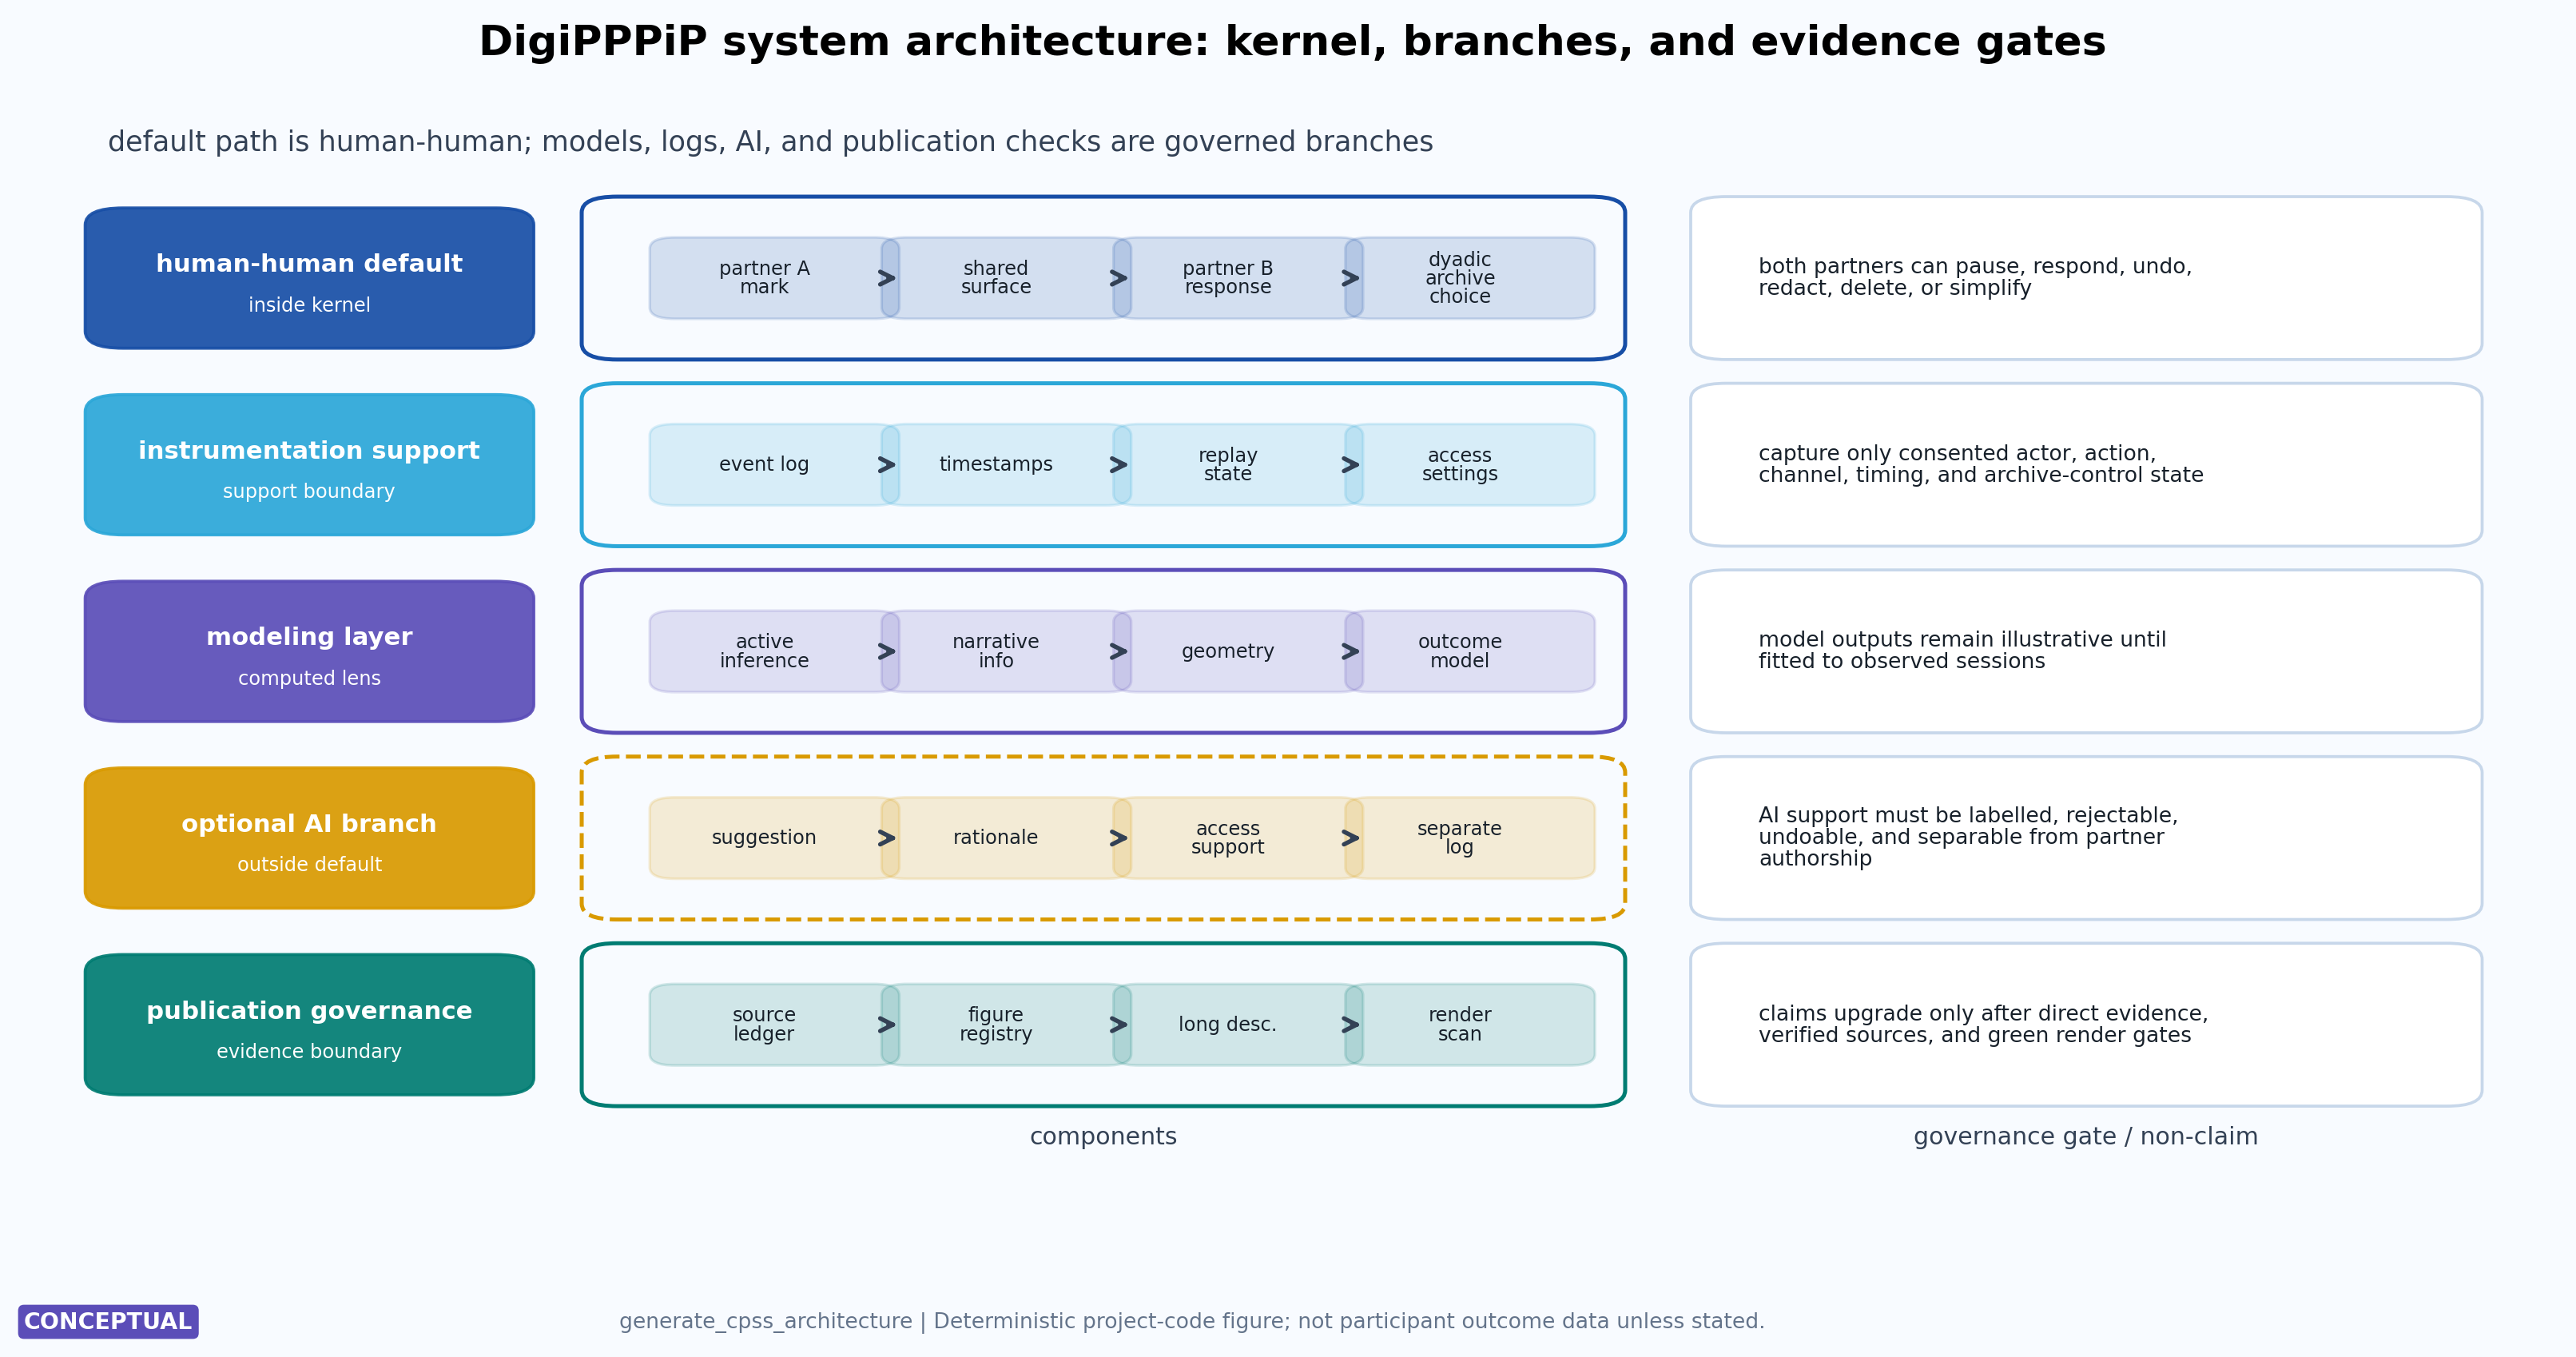
\includegraphics[width=0.95\linewidth,height=0.46\textheight,keepaspectratio,alt={DigiPPPiP system architecture with a human-human default lane, instrumentation support, computed modeling layer, optional AI branch, and publication-governance boundary. The figure is generated by generate\_cpss\_architecture() from src/systems\_governance.py; read the left badges as boundary status, the middle blocks as components, and the right boxes as governance gates or non-claims. It supports the cyberphysical argument that system boundaries must be explicit before features are interpreted. The diagram is conceptual, and validation would require observing how real interface changes affect partner behavior, consent, access, and archive control.}]{../figures/cpss_architecture.png}
\caption{DigiPPPiP system architecture with a human-human default lane,
instrumentation support, computed modeling layer, optional AI branch,
and publication-governance boundary. The figure is generated by
\protect\breaktt{generate\_cpss\_architecture()} from
\protect\breaktt{src/systems\_governance.py}; read the left badges as
boundary status, the middle blocks as components, and the right boxes as
governance gates or non-claims. It supports the cyberphysical argument
that system boundaries must be explicit before features are interpreted.
The diagram is conceptual, and validation would require observing how
real interface changes affect partner behavior, consent, access, and
archive control.}\label{fig:cpss_architecture}
\end{figure}

\breakseq{[@fig:cyberphysical\_spectrum]} positions the modes as affordance
trade-offs rather than replacements. Physical-only PPPiP preserves
haptic richness and place grounding. Remote digital modes extend
geographic reach and accessibility. Hybrid modes are especially
important because they let one partner keep a material surface while the
shared artifact remains digitally visible, versioned, and transportable.

\begin{figure}
\centering
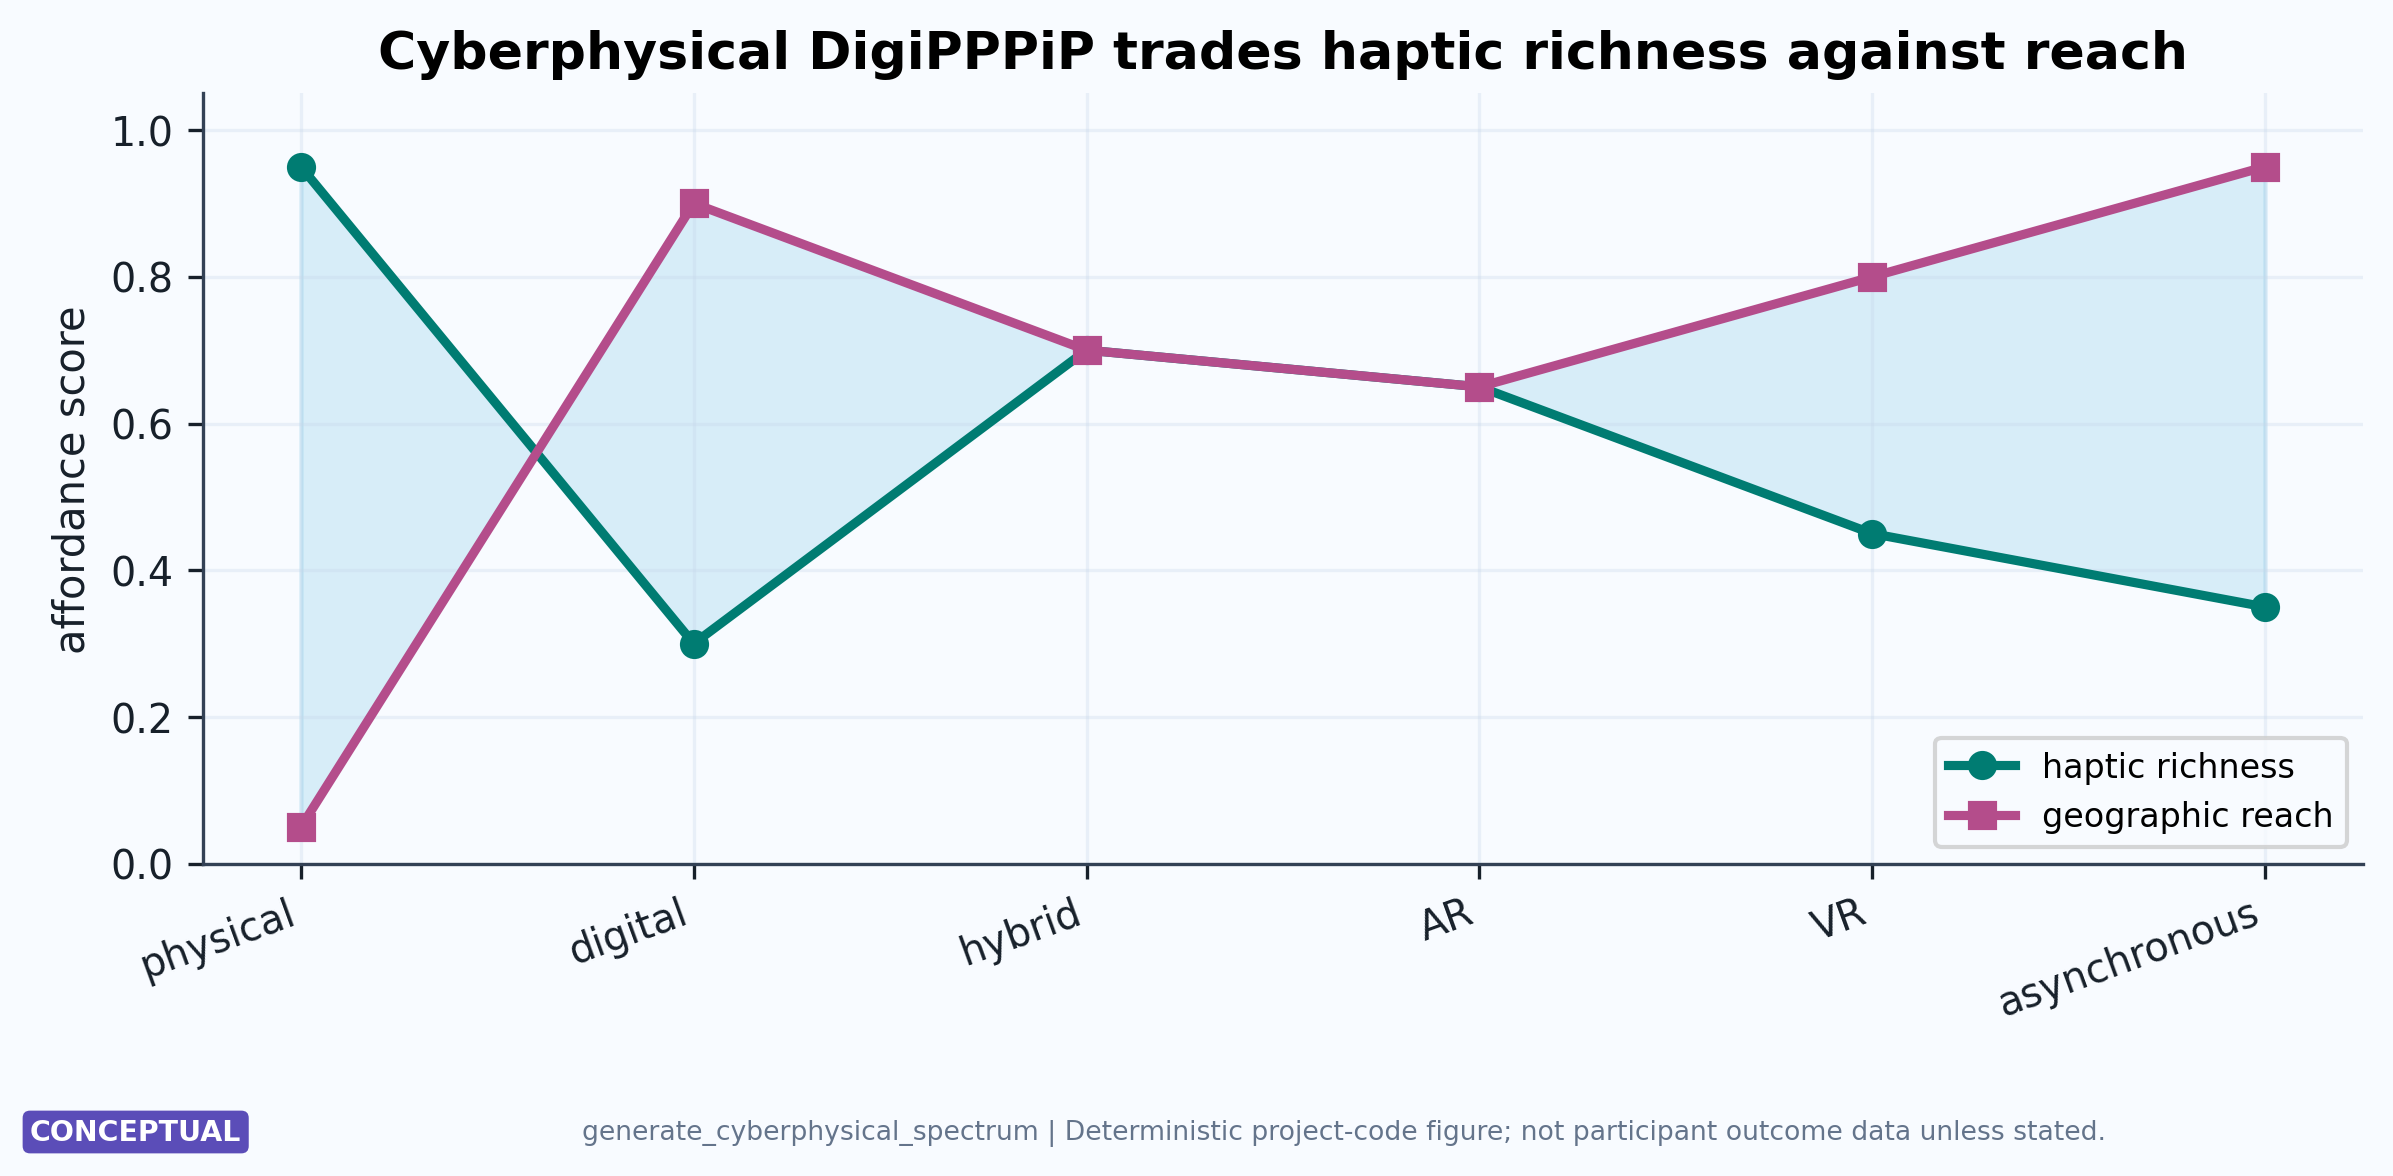
\includegraphics[width=0.9\linewidth,height=0.46\textheight,keepaspectratio,alt={Cyberphysical affordance spectrum for physical, digital, hybrid, AR, VR, and asynchronous drawing modes. Scores are conceptual design variables generated by generate\_cyberphysical\_spectrum(); read the green and purple lines as contrasting affordances for haptic richness and geographic reach, with the filled area marking trade-off space. The plot supports modality selection, not superiority claims; measured user outcomes would be needed to calibrate the scores.}]{../figures/cyberphysical_spectrum.png}
\caption{Cyberphysical affordance spectrum for physical, digital,
hybrid, AR, VR, and asynchronous drawing modes. Scores are conceptual
design variables generated by
\protect\breaktt{generate\_cyberphysical\_spectrum()}; read the green and
purple lines as contrasting affordances for haptic richness and
geographic reach, with the filled area marking trade-off space. The plot
supports modality selection, not superiority claims; measured user
outcomes would be needed to calibrate the
scores.}\label{fig:cyberphysical_spectrum}
\end{figure}

The minimum viable substrate is not ``a digital drawing app.'' It is any
arrangement that lets partner action become visible as a shared mark
while preserving enough timing, authorship, and consent context for the
other partner to respond. A high-resolution tablet can fail that test if
notifications, menus, opaque storage policies, or AI prompts pull
attention away from the dyad. A photographed paper exchange can satisfy
it if the image, timing, and response loop remain clear. This is the
first-principles reason the framework treats cyberphysical modes as
affordance configurations rather than a progress ladder.

This substrate shift changes the research problem. The central question
is no longer whether digital drawing is equivalent to paper drawing. A
more useful question is which relational affordance a pair needs in a
given context: immediacy, haptics, accessibility, distance, persistence,
privacy, or place anchoring. The taxonomy in \breakseq{[@sec:taxonomy]} gives
those choices a stable vocabulary, and the protocol in
\breakseq{[@sec:methods\_protocol]} defines what must be logged before such
affordances can be compared.
\end{frame}

\end{document}
